\documentclass[12pt]{article}
\usepackage{amssymb, amsmath, amsfonts, bm, graphicx, geometry}
\usepackage{tabularx, booktabs, float, enumitem, multicol, mathtools}
\usepackage{enumitem}
\setlist[itemize,1]{label=$\bullet$}
\setlist[itemize,2]{label=--}
\setlist[itemize,3]{label=$\circ$}
\setlist[itemize,4]{label=$\cdot$}
\usepackage{parskip} % Auto-manages paragraph spacing and removes indentations
\usepackage{siunitx}  % Eases typesetting of numbers and units
\usepackage[hidelinks]{hyperref}

% US customary units
\DeclareSIUnit{\inch}{in}
\DeclareSIUnit{\foot}{ft}
\DeclareSIUnit{\yard}{yd}
\DeclareSIUnit{\mile}{mi}

\DeclareSIUnit{\slug}{slug}
\DeclareSIUnit{\lbm}{lbm}
\DeclareSIUnit{\lbf}{lbf}

\DeclareSIUnit{\psi}{psi}
\DeclareSIUnit{\psf}{psf}

\DeclareSIUnit{\gallon}{gal}
\DeclareSIUnit{\quart}{qt}
\DeclareSIUnit{\fahrenheit}{F}
\DeclareSIUnit{\rankine}{R}
\sisetup{
    per-mode = fraction
}
\usepackage{soul}
\usepackage{mathrsfs}

\geometry{margin=1in}

% Uppercase Volume with thicker, higher line
\newcommand{\vol}{\mathord{\text{\ooalign{\hidewidth $V$\hidewidth\cr\kern-0.5pt\raisebox{0.8ex}{\rule[0pt]{1em}{0.5pt}}}}}}

% Lowercase Volume with built-in shifts
\newcommand{\svol}{%
  \mathord{\text{\ooalign{%
    \hfil$v$\hfil\cr
    \hfil\rule[0.6ex]{0.8em}{0.5pt}\hfil
  }}}%
}

\begin{document}

\begin{center}
{\LARGE ESC-340 Fluid Mechanics \& Flow Systems Notes\par}
\end{center}
\hrule
\vspace{1.5em}
\begin{center}
    {\LARGE\bfseries Fluid Kinematics\par}
\end{center}
In this chapter, we will study fluid motion without considering the forces that causes the motion. In other words, we will only look at the velocity and acceleration of a fluid but not the pressure or other forces that causes it. In other words, its fluid kinematics.
\section*{\fbox{4.1 The velocity field}}
\vspace{-2em}
\addcontentsline{toc}{section}{4.1 The velocity field}
\begin{minipage}[c]{0.5\textwidth}
    A fluid's motion can be described by its \textit{velocity field}, which defines the velocity of a fluid at every position and time:
    \[\vec{V}=u(x,y,z,t)\hat{\imath} + v(x,y,z,t)\hat{\jmath} + w(x,y,z,t)\hat{k}\]
\end{minipage}
\hfill
\begin{minipage}[c]{0.45\textwidth}
    \centering
    \includegraphics[width=\linewidth]{velocity vector.jpeg}
\end{minipage}
For example, the velocity field at a specific instant (constant $t$) can be shown as:
\begin{center}
    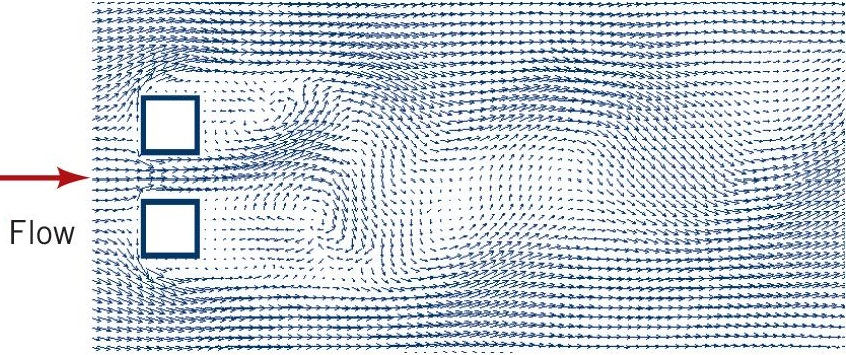
\includegraphics[width=0.6\linewidth]{velocity field.jpeg}
\end{center}
\subsection*{Eulerian and Lagrangian Flow Descriptions}
There are two general approaches for analyzing fluid mechanics problems:
\begin{itemize}
    \item \textbf{Eulerian Method:}\\
    The Eulerian method focuses on fixed regions in space through which the fluid flows. In this approach, we visualize the fluid motion by using fields of velocity, pressure, and other properties at specific points in space. For example, we can analyze the pressure field in a fixed region around an airfoil:
    \begin{center}
        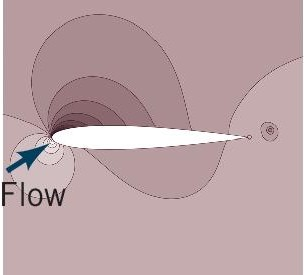
\includegraphics[width=0.25\linewidth]{eulerian.jpeg}
    \end{center}
    \item \textbf{Lagrangian Method:}\\
    Unlike the Eulerian method, the Lagrangian method tracks individual fluid particles as they move through space and time. In this approach, we follow the trajectory of a specific fluid particle and analyze its properties along its path. For example, to analyze the behavior of smoke exiting a chimney:
    \begin{center}
        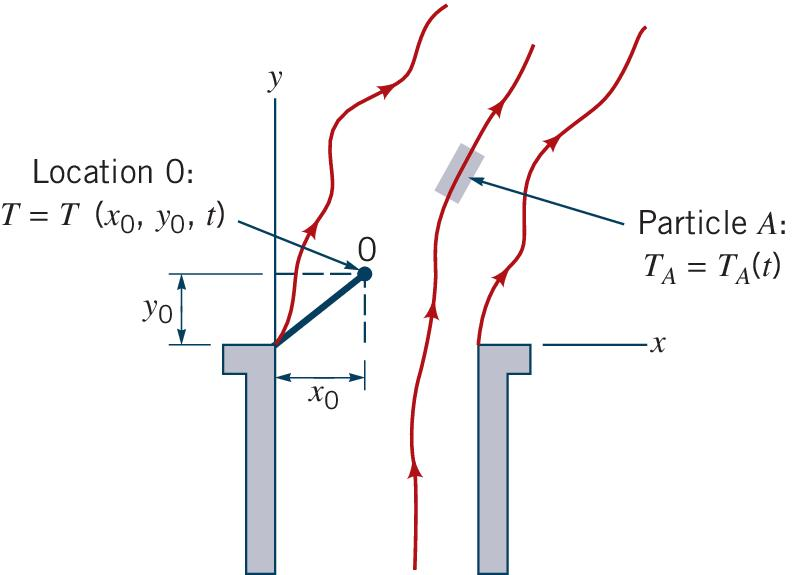
\includegraphics[width=0.4\linewidth]{lagrangian.jpeg}
    \end{center}
    The Eulerian method would involve measuring the temperature with a thermometer at a fixed point $0 = (x_0, y_0)$, obtaining $T(x_0, y_0, t)$, while the Lagrangian method would involve following a specific smoke particle $A$ and measuring its temperature along its path, obtaining $T_A(t)$.
\end{itemize}
It is important to note that both approaches are valid and are interchangeable, but generally the Eulerian method is more convenient.
\subsection*{Steady and Unsteady Flows}
In the previous sections, we typically assumed steady flow, where the velocity at a given point does not vary with time ($\partial \vec{V}/\partial t = 0$). Some types of unsteady flows include:
\begin{itemize}
    \item \textbf{Non-periodic flow:} unsteady flow that does not repeat cyclically, such as water accelerating in a pipe when a valve is opened.
    \item \textbf{Periodic flow:} unsteady flow that repeats cyclically
    \item \textbf{Random flow:} unsteady flow that is unpredictable, such as turbulent flow.
\end{itemize}
Note that steady flow does not mean constant fluid velocity, as it can still vary across space, just not with time.
\subsection*{Streamlines, Streaklines, and Pathlines}
These are ways to help in the visualization of fluid motion. Typically streamlines are used often in analytical work, while streaklines and pathlines are used in experimental work.
\begin{itemize}
    \item \textbf{Streamline:}\\
    A streamline is a line that is everywhere tangent to the velocity vector of the flow. \textit{If the flow is steady, the streamlines are fixed lines in space.} For unsteady flows the streamlines may change shape with time.\\
    \begin{minipage}[c]{0.6\textwidth}
    For two-dimensional flow, the streamlines can be defined by the equation:
    \[\frac{dy}{dx} = \frac{v}{u}\]
    By definition, the velocity vector is tangent to the streamline, so the slope of the streamline is equal to the ratio of the velocity components \textit{at every point}.
\end{minipage}
\hfill
\begin{minipage}[c]{0.25\textwidth}
    \centering
    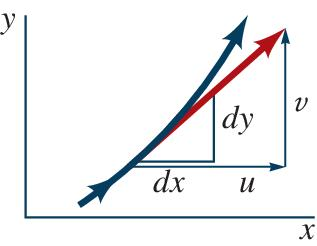
\includegraphics[width=\linewidth]{streamline.jpeg}
\end{minipage}
\begin{center}
    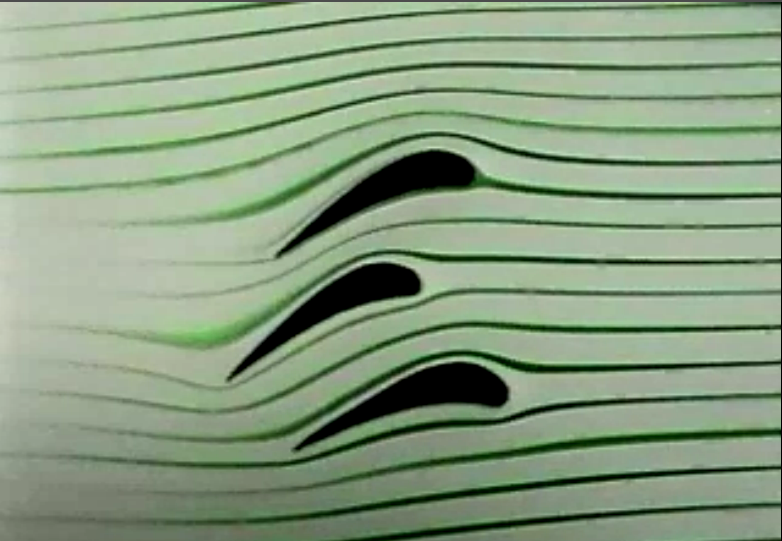
\includegraphics[width=0.5\linewidth]{streamline 1.png}
\end{center}
\item \textbf{Streakline:}\\
A streakline consists of all the particles in a flow that \hl{have passed through the same point in space.} Experimentally, streaklines can be visualized by continuously injecting dye into the flow at a fixed point and observing the path of the dye particles.
\begin{center}
    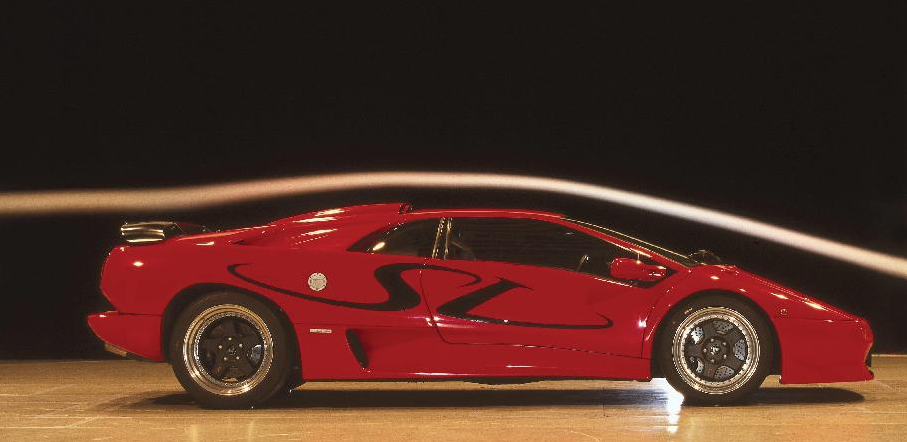
\includegraphics[width=0.5\linewidth]{Streakline.png}
\end{center}
\item \textbf{Pathline:}\\
A pathline is the line traced out by a given particle as it flows from one point to another. The pathline is a Lagrangian concept that can be produced in the laboratory by marking a fluid particle (dyeing a small fluid element) and taking a time exposure photograph of its motion. (Like taking a long exposure photo of a light moving in the dark.)
\end{itemize}
For steady flow, the streamlines, streaklines, and pathlines are identical. For unsteady flow, they are different.
\newpage
\section*{\fbox{4.2 The Acceleration Field}}
\addcontentsline{toc}{section}{4.2 The Acceleration Field}
For the infrequently used Lagrangian method, the acceleration of a fluid particle is the same as in solid body mechanics: $\vec{a} = \vec{a} (t)$. For the Eulerian method, we describe the \textit{acceleration field}, just like the velocity field previously.
\subsection*{Acceleration Field}
Consider the velocity of a single fluid particle $A$ moving along its pathline, where $\vec{r}_A$ is the position vector of the particle $A$ at time $t$. The velocity of the particle is given by:
\[\vec{V}_A = \vec{V}_{A}(\vec{r}_A,t) = \vec{V}_{A}\big(\,x_A(t), y_A(t), z_A(t),t\,\big)\]
\begin{center}
    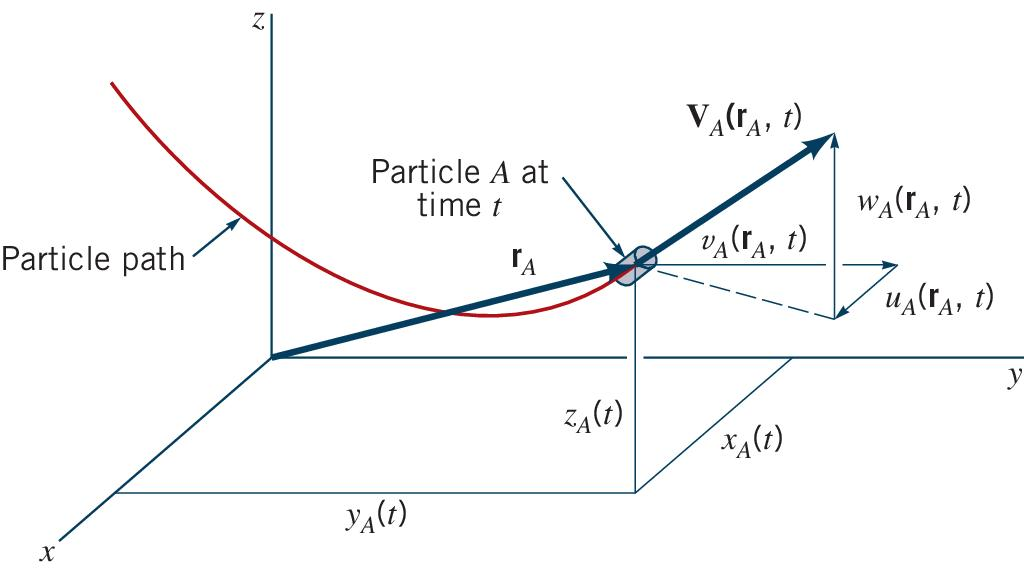
\includegraphics[width=0.7\linewidth]{velocity of particle.jpeg}
\end{center}
By definition, the acceleration of the fluid particle is the time derivative of its velocity:
\[\vec{a}_A = \frac{d\vec{V}_A}{dt}\]
By chain rule:
\[\frac{d\vec{V}_A}{dt}=\frac{\partial\vec{V}_A}{\partial t}+\frac{\partial\vec{V}_A}{\partial x}\frac{dx_A}{dt}+\frac{\partial\vec{V}_A}{\partial y}\frac{dy_A}{dt}+\frac{\partial\vec{V}_A}{\partial z}\frac{dz_A}{dt}\]
Using the velocity components given by $u_A = dx_A/dt$, $v_A = dy_A/dt$, and $w_A = dz_A/dt$, we can rewrite the acceleration as:
\[\vec{a}_A = \frac{\partial\vec{V}_A}{\partial t} + u_A\frac{\partial\vec{V}_A}{\partial x} + v_A\frac{\partial\vec{V}_A}{\partial y} + w_A\frac{\partial\vec{V}_A}{\partial z}\]
\hl{This statement is valid for any particle, we can drop the subscript $A$ and define the acceleration field as:}
\[\boxed{\vec{a} = \frac{\partial\vec{V}}{\partial t} + u\frac{\partial\vec{V}}{\partial x} + v\frac{\partial\vec{V}}{\partial y} + w\frac{\partial\vec{V}}{\partial z}}\]
\newpage
With the corresponding scalar components:
\begin{align*}
a_x &= \frac{\partial u}{\partial t} + u\frac{\partial u}{\partial x} + v\frac{\partial u}{\partial y} + w\frac{\partial u}{\partial z}\\
a_y &= \frac{\partial v}{\partial t} + u\frac{\partial v}{\partial x} + v\frac{\partial v}{\partial y} + w\frac{\partial v}{\partial z}\\
a_z &= \frac{\partial w}{\partial t} + u\frac{\partial w}{\partial x} + v\frac{\partial w}{\partial y} + w\frac{\partial w}{\partial z}
\end{align*}
Note that the equation for the acceleration field describes two different sources of acceleration:
\[\vec{a}=\underbrace{\frac{\partial\vec{V}}{\partial t}}_{\text{Local acceleration}}+\underbrace{u\frac{\partial\vec{V}}{\partial x}+v\frac{\partial\vec{V}}{\partial y}+w\frac{\partial\vec{V}}{\partial z}}_{\text{Convective acceleration}}\]
Where:
\begin{itemize}
    \item \textbf{Local acceleration} describes velocity changes with time, \hl{which is only present in unsteady flows}.
    \begin{center}
        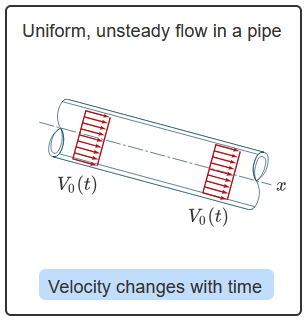
\includegraphics[width=0.3\linewidth]{local acceleration.png}
    \end{center}
    \item \textbf{Convective acceleration} describes velocity changes with position, which is present in both steady and unsteady flows.
    \begin{center}
        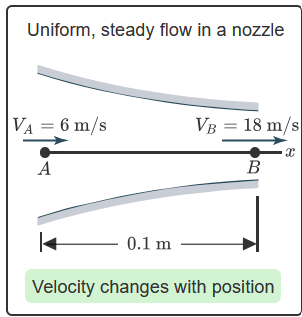
\includegraphics[width=0.3\linewidth]{convective acceleration.png}
    \end{center}
\end{itemize}
\newpage
\subsection*{Material Derivative Defined}
The equation for the acceleration field can be expressed in a more compact form by defining the \textit{material derivative}:
\[\vec{a} = \frac{D\vec{V}}{Dt}\]
Where the material derivative is a differential operator defined as:
\[\boxed{\frac{D()}{Dt}\equiv\frac{\partial()}{\partial t}+u\frac{\partial()}{\partial x}+v\frac{\partial()}{\partial y}+w\frac{\partial()}{\partial z}}\]
Or shorthand notation:
\[\boxed{\frac{D()}{Dt}=\frac{\partial()}{\partial t}+(\vec{V}\cdot\vec{\nabla})()}\]
Note that the gradient operator $\vec{\nabla}$ is defined as:
\[\vec{\nabla}()=\frac{\partial()}{\partial x}\hat{\imath}+\frac{\partial()}{\partial y}\hat{\jmath}+\frac{\partial()}{\partial z}\hat{k}\]
So 
\[\vec{V}\cdot\vec{\nabla}()=u\frac{\partial()}{\partial x}+v\frac{\partial()}{\partial y}+w\frac{\partial()}{\partial z}\]
\hl{The material derivative is not just for the acceleration field, it can be applied to any flow property, such as pressure, temperature, or density.} The material derivative of any variable is the rate at which that variable changes with time for a given particle \hl{\textit{as seen by one moving along with the fluid}}.\\\\
For example, the material derivative of temperature $T$ describes how temperature changes with time as a fluid particle moves along its pathline in the candle flame:
\begin{center}
    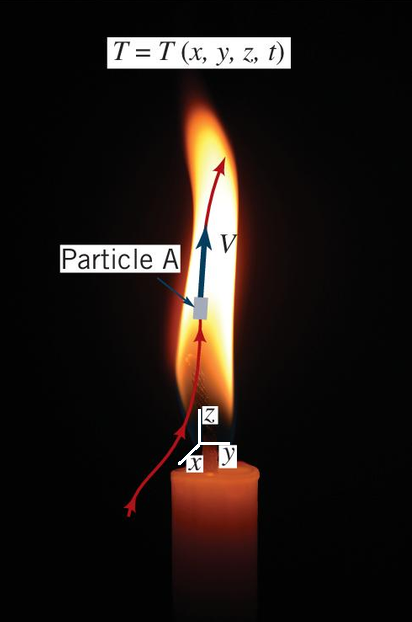
\includegraphics[width=0.3\linewidth]{material deriv of temp.png}
\end{center}
\newpage
\subsection*{Acceleration with Streamline Coordinates}
As defined previously in section 3.1, the streamline coordinate system is defined by the unit vectors $\hat{s}$ along the streamline and $\hat{n}$ normal to the streamline:
\begin{center}
    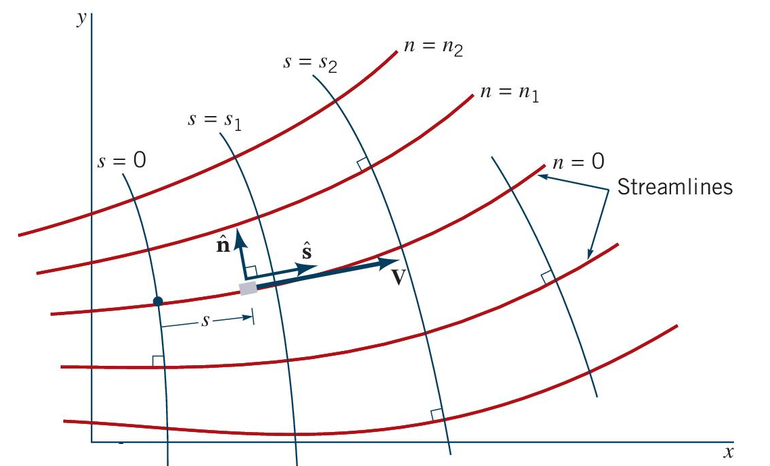
\includegraphics[width=0.7\linewidth]{streamline coords.png}
\end{center}
Where $\vec{V}=V\hat{s}$ for steady, 2D flow. \hl{Since we are following a fluid particle along its streamline, we use the material derivative to determine the acceleration experienced by the particle as it moves through the flow.} Taking the material derivative of the velocity vector:
\[\vec{a}=\frac{D(V\hat{s})}{Dt}=\frac{DV}{Dt}\hat{s}+V\frac{D\hat{s}}{Dt}\]
\[\vec{a}=\left(\frac{\partial V}{\partial t}+\frac{\partial V}{\partial s}\frac{ds}{dt}+\frac{\partial V}{\partial n}\frac{dn}{dt}\right)\hat{s}+V\left(\frac{\partial\hat{s}}{\partial t}+\frac{\partial\hat{s}}{\partial s}\frac{ds}{dt}+\frac{\partial\hat{s}}{\partial n}\frac{dn}{dt}\right)\]
Applying the chain rule to both terms, and noting that for steady flow:
\begin{itemize}
    \item $\partial V/\partial t = \partial \hat{s}/\partial t=0$: for steady flow.
    \item $ds/dt=V$: the particle moves along the streamline at speed $V$.
    \item $dn/dt=0$: the particle remains on its streamline ($n =$ constant).
\end{itemize}
The acceleration simplifies to
\[\vec{a}=\underbrace{V\frac{\partial V}{\partial s}\hat{s}}_{\text{Tangential acceleration}}+\underbrace{V^2\frac{\partial\hat{s}}{\partial s}}_{\text{Normal acceleration}}\]
Since the rate of change of the tangent unit vector along a curved streamline is
\[\frac{\partial\hat{s}}{\partial s}=\frac{1}{\mathscr{R}}\hat{n}\]
\hl{This is the same result as in section 3.1}
\newpage
\section*{\fbox{4.3 Control Volume and System Representations}}
\addcontentsline{toc}{section}{4.3 Control Volume and System Representations}
First a note on terminology between systems and control volumes in thermodynamics and fluid mechanics:
\begin{center}
\begin{tabular}{lll}
    \hline
    \textbf{Concept} & \textbf{Thermodynamics} & \textbf{Fluid Mechanics} \\
    \hline
    Fixed amount of matter & Closed system (control mass) & System \\[8pt]
    \begin{tabular}[t]{@{}l@{}}
        Specified region in space where\\
        mass can enter or exit
    \end{tabular}
    & Open system (control volume) & Control volume \\
    \hline
\end{tabular}
\end{center}
\textit{A system follows the matter, while a control volume follows a region in space.}
\subsection*{Types of Control Volumes}
Some typical control volumes used in fluid mechanics are shown below. (a) is a fixed control volume within a pipe with fluid flowing through it. (b) is a moving control volume that remains fixed relative to a moving object, in this case, a jet engine. Note that the fluid initially contained within the control volume at $t_1$ is not necessarily the same fluid contained within it at $t_2$, since fluid continuously enters and leaves the engine. (c) is a deforming control volume that contains the fluid within a deflating balloon.
\begin{center}
    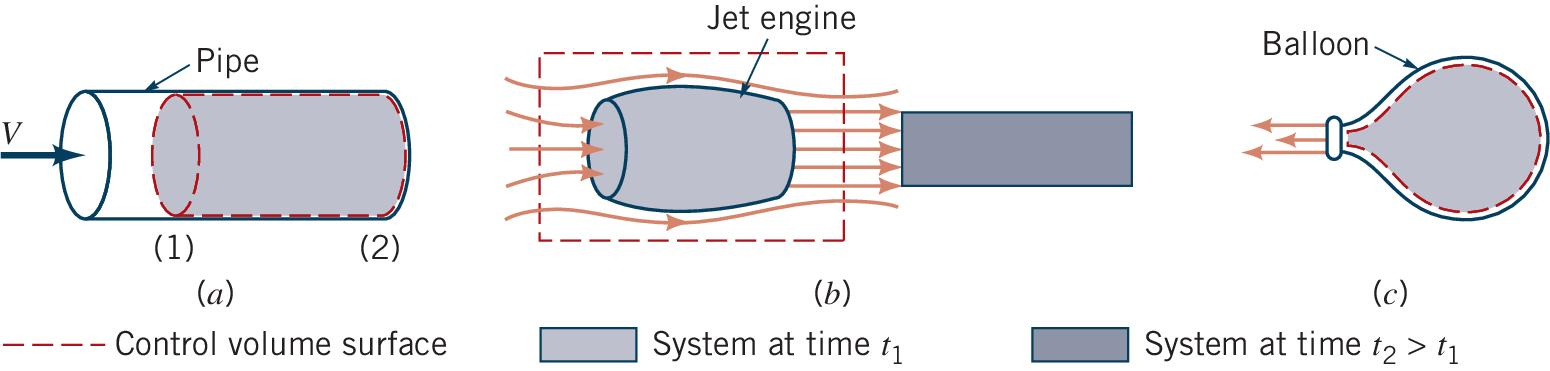
\includegraphics[width=0.75\linewidth]{control volumes.jpeg}
\end{center}
Ideally, when approaching a control volume problem, we want to define the control volume such that \hl{the parameters along the control surface are either known, reasonably approximated, or are the unknowns we wish to determine}, while allowing us to neglect complex internal effects.
\begin{center}
    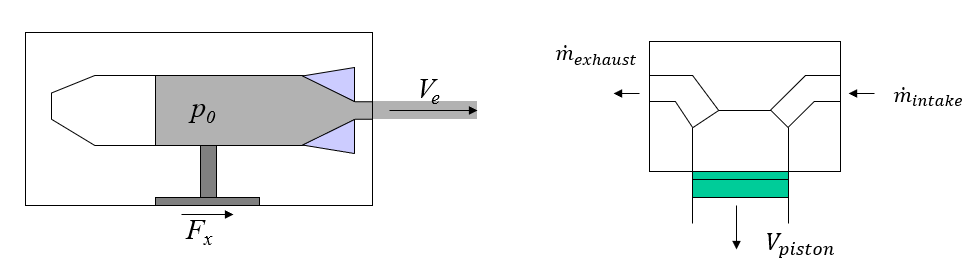
\includegraphics[width=0.75\linewidth]{control volumes 2.png}
\end{center}
A \textbf{control surface} is the boundary of a control volume, which can be real or imaginary, just like in thermodynamics.
\newpage
\section*{\fbox{4.4 The Reynolds Transport Theorem}}
\addcontentsline{toc}{section}{4.4 The Reynolds Transport Theorem}
In a single line, \hl{the Reynolds Transport Theorem is an analytical tool that connects changes in the system (control mass) with changes in the control volume.} This allows us to analyze fluid effects on a particular object or volume in space, such as force of a water jet on a plate.\\\\
Conservation laws, such as Newton's second law, are typically expressed in terms of a system (with fixed mass). However, most fluid mechanics problems are more easily analyzed using a control volume, so we use the Reynolds Transport Theorem to convert system equations into control volume equations.\\\\
Recall that a system \textit{follows} a fixed mass of fluid (or a fixed collection of particles) as it moves through space and time.
\subsection*{Intensive vs Extensive Fluid Properties}
Recall from thermodynamics that extensive properties depend on the size or mass of a system, while intensive properties do not. \hl{By normalizing an extensive property $B$ by mass, we obtain an intensive (or specific) property $b=B/m$}, which is intensive and independent of the amount of matter present.\\\\
This is very useful for control volume analysis, \hl{where mass flows across the control surface, carrying its associated properties with it.} Thus, we can determine the rate at which a property is transported by multiplying the specific property by the mass flow rate.\\\\
\underline{Note:} Some properties, such as temperature and pressure, are already intensive since they are independent of the amount of matter present. However, other properties, such as momentum and energy, are extensive and can be normalized by mass to obtain intensive properties.\\\\
Thus, we can say that the \textit{total amount of some property $B$ within a system is}
\[B_{\text{sys}} = \int_{\text{sys}} b \, dm = \int_{\text{sys}} \rho b\,d\vol\]
Where $b$ is the intensive property associated with the extensive property $B$, $\rho$ is the fluid density, and $d\vol$ is an infinitesimal volume element. \hl{The limits of integration cover the entire system (sums over all the particles in the system). \textit{This is usually a moving volume.}}\\\\
\underline{Note:} The parameters $B$ and $b$ can be both vector or scalar quantities!\\\\
\textbf{Time Rate of Change of a System Property}\\
Most laws governing the fluid motion are expressed in terms of the time rate of change of a system property. For example, the rate of change of momentum is equal to the net force acting on the system, or the rate of change in mass is equal to the net mass flow into or out of the system.
\newpage
Thus, defining the time rate of change of an extensive property $B$ \textit{within a system} using the intensive property $b$:
    \[\frac{dB_{\text{sys}}}{dt} =  \frac{d}{dt}\left(\int_{\text{sys}} \rho b\,d\vol\right)\]
Equivalently, we can make a similar statement for the time rate of change of an extensive property $B$ \hl{within a control volume}:
\[\frac{dB_{C\vol}}{dt} =  \frac{d}{dt}\left(\int_{C\vol} \rho b\,d\vol\right)\]
While the forms of the equations are similar, \hl{they have mathematically different limits of integration!} This is because typically, the control volume is fixed in space, while the system is a moving volume that follows a fixed collection of fluid particles. Furthermore, \hl{the control volume can have mass entering or leaving it, while the system has a fixed mass,} so the time rates of change would not necessarily be equal. \textit{Reynold's transport theorem gives us a way to relate these two derivatives!}\\\\
\underline{Example:}\\
Consider the system to be the fluid contained within a tank at $t=0$ when the valve is opened. The control volume is the fixed volume of the tank.
\begin{center}
    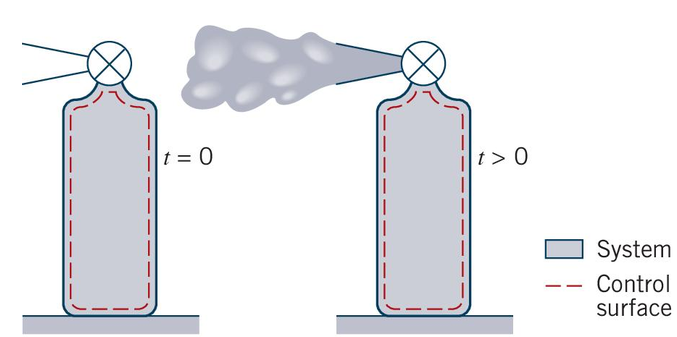
\includegraphics[width=0.5\linewidth]{control volume example.png}
\end{center}
If mass is conserved, then the time rate of change of mass within the system is zero:
\[\frac{d}{dt}\left(\int_{\text{sys}} \rho b\,d\vol\right) =0\]
But since mass has exited the control volume, the time rate of change of mass within the control volume is negative:
\[\frac{d}{dt}\left(\int_{C\vol} \rho b\,d\vol\right) < 0\]
\noindent
\begin{minipage}[c]{0.8\textwidth}
    \textit{Intuitively, this is all obvious stuff, but it's very important to know the difference between the two definitions. Otherwise, Reynolds would be sad...}
\end{minipage}%
\hfill
\begin{minipage}[c]{0.15\textwidth}
    \centering
    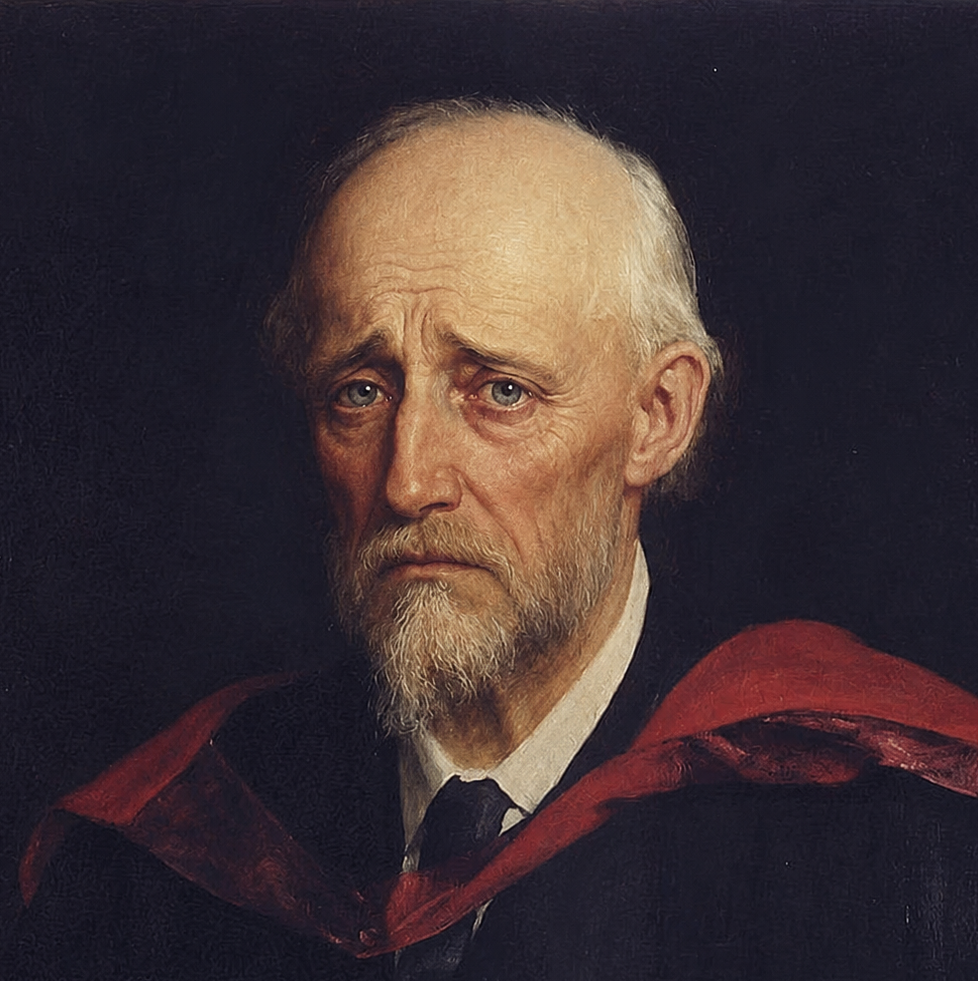
\includegraphics[width=\linewidth]{sad reynold.png}
\end{minipage}
\newpage
\subsection*{Derivation of the Reynolds Transport Theorem}
The goal of the Reynolds Transport Theorem is to \hl{relate the rate of change of a property of a moving system to the changes occurring within a control volume}.\\\\
To do this, we can initially define a system that is \textit{entirely contained within and coincides with the control volume}. If the fluid particles that make up the system have some velocity, then the system will move relative to the \textit{fixed} control volume over a small time interval. By accounting for the fluid entering and leaving the control volume, we can express the rate of change of the system's property.\\\\
\underline{Note:} While we initially derive the Reynolds Transport Theorem for one-dimensional flow through a fixed control volume, we can generalize the resulting equation to account for arbitrary flow directions and nonuniform flow across the control surface.\\\\
Consider the following system and control volume of a fluid flowing through a variable area pipe:
\begin{center}
    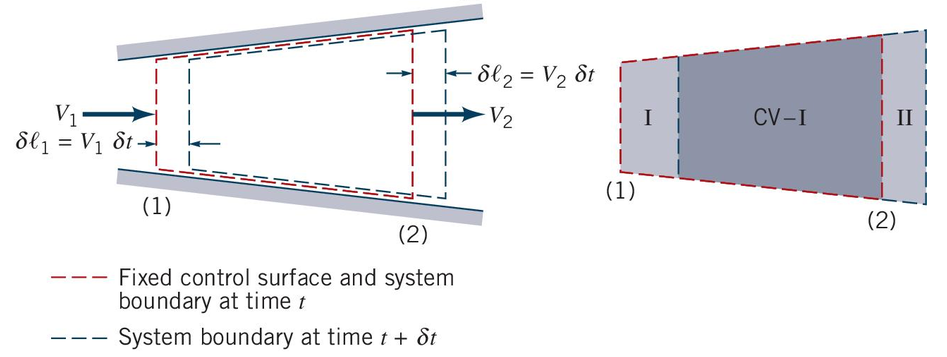
\includegraphics[width=0.85\linewidth]{reynolds transport theorem.png}
\end{center}
\textbf{Derivation Set up}
\begin{itemize}
    \item The control volume is fixed between sections (1) and (2), while the fluid velocity normal to the control surfaces is $V_1$ and $V_2$ respectively.
    \item The system of fluid particles is initially contained inside the control volume at initial time $t$.
\end{itemize}
A short time later, at time $t+\delta t$, the system has moved slightly to the right of the control volume:
\begin{itemize}
    \item The fluid particles initially at section (1) have moved a distance $\delta \ell_1 = V_1 \delta t$ to the right
    \item The fluid particles initially at section (2) have moved a distance $\delta \ell_2 = V_2 \delta t$ to the right
\end{itemize}
Thus, we define the following volumes of the fluid at time $t+\delta t$:
\begin{itemize}
    \item \textbf{C$\vol$}: The volume of the fixed control volume, which is the same as at time $t$.
    \item \textbf{II}: The volume of fluid that exited the control volume (the outflow through section (2)) during the time interval $\delta t$.
    \item \textbf{I}: The volume of fluid that entered the control volume (the inflow through section (1)) during the time interval $\delta t$.
\end{itemize}
The system at time $t+\delta t$ is now composed of the following three volumes as shown in the diagram previously:
\[\text{SYS} = (\text{C$\vol$} - \text{I}) +\text{II}\]
The control volume is fixed, so C$\vol$ = C$\vol$.\\\\
\textbf{Using changes in fluid volume to derive statements of $B$}\\
Now, we find the relationships of the extensive property $B$ for the system and control volume at time $t+\delta t$:
\begin{itemize}
    \item By definition, the extensive property $B$ at time $t$ is equal for both the system and control volume:
    \[B_{\text{sys}}(t) = B_{C\vol}(t)\]
    \item The extensive property $B$ at time $t+\delta t$ for the system can be expressed by the sum of the extensive properties of the three volumes:
    \[B_{\text{sys}}(t+\delta t) = B_{C\vol}(t+\delta t) - B_{\text{I}}(t+\delta t) + B_{\text{II}}(t+\delta t)\]
\end{itemize}
\textbf{Finding the time rate of change in $B$}\\
Now, let's find the time rate of change of the extensive property $B$ for the system. Starting with a forward finite difference approximation and then substituting the previous eqns:
\[
\frac{\delta B_{\mathrm{sys}}}{\delta t}
= \frac{B_{\mathrm{sys}}(t+\delta t)-B_{\mathrm{sys}}(t)}{\delta t}
= \frac{\big[B_{\mathrm{c\vol}}(t+\delta t)-B_{\mathrm{I}}(t+\delta t)+B_{\mathrm{II}}(t+\delta t)\big]-\big[B_{C\vol}(t)\big]}{\delta t}
\]
Rearranging the terms, we have:
\[\frac{\delta B_{\mathrm{sys}}}{\delta t} = \frac{B_{\mathrm{c\vol}}(t+\delta t)-B_{C\vol}(t)}{\delta t} - \frac{B_{\mathrm{I}}(t+\delta t)}{\delta t} + \frac{B_{\mathrm{II}}(t+\delta t)}{\delta t}\]
\underline{Important Note:} This is a key step in the derivation, relating changes in the system's property to those in the control volume. The system's change equals the change within the control volume, minus the property entering and plus the property leaving with the fluid.\hl{ Intuitively, this makes sense because extensive properties depend on the amount of matter present, which can be related to the volume it occupies. Thus, we can understand changes in these properties through the volumes of fluid entering and leaving the control volume.}
\newpage
Taking the limit as $\delta t \to 0$:
\begin{itemize}
    \item Left-hand side:
    \[\lim_{\delta t \to 0} \frac{\delta B_{\mathrm{sys}}}{\delta t} = \frac{DB_{\mathrm{sys}}}{Dt}\]
    Note that mathematically, the limit gives the first-order time derivative of $B_{\mathrm{sys}}$. \hl{However, we use the material derivative notation to emphasize that the derivative describes the rate of change of $B$ as seen by an observer that moves with the fluid particles that constitute the system.}
    \item Right-hand side (first term):
    \[
\lim_{\delta t \to 0}\frac{B_{\mathrm{C\vol}}(t+\delta t)-B_{\mathrm{C\vol}}(t)}{\delta t}=\frac{\partial B_{\mathrm{C\vol}}}{\partial t}
\]
\[\frac{\partial B_{\mathrm{C\vol}}}{\partial t} = \frac{\partial}{\partial t}\left(\int_{C\vol} \rho b\, d\vol\right)\]
Note that the integral $\int_{C\vol} \rho b\, d\vol$ represents the total amount of property $B$ within the fixed control volume. \hl{Since the control volume is fixed, its boundaries don't change, so the limits of integration are constant.} Therefore, the time derivative $\partial B_{\mathrm{C\vol}}/\partial t$ is positive when the total amount of $B$ within the control volume increases, or in other words, when the integral "accumulates" more of the property $B$ over time.
\begin{itemize}
    \item Examples for when $\rho$ is increasing:
    \begin{itemize}
        \item \textbf{Mass ($B=M$, $b=1$):} Air is pumped into a rigid tank, increasing its density $\rho$ and therefore its total mass.
        \item \textbf{Momentum ($B=\vec{P}$, $b=\vec{V}$):} Air is compressed while maintaining its velocity, increasing $\rho$ and therefore its total momentum.
    \end{itemize}

    \item Examples for when $b$ is increasing:
    \begin{itemize}
        \item \textbf{Momentum ($B=\vec{P}$, $b=\vec{V}$):} Fluid accelerates within a pipe, increasing its velocity $\vec{V}$ and therefore its momentum.
        \item \textbf{Energy ($B=E$, $b=e$):} Water is heated, increasing its specific energy $e$ and therefore its total energy.
    \end{itemize}

    \item Example for when fluid occupies an increasing portion of the control volume:
    \begin{itemize}
        \item \textbf{Mass ($B=M$, $b=1$):} Water fills an initially empty tank, increasing the volume occupied by water and therefore its total mass, even though the water's density remains constant.

Consider a fixed control volume consisting of a tank, with constant cross-sectional area $A$, total height $H$, and water level $h(t)$. The water density field is defined as:
\[
\rho(z,t)=
\begin{cases}
\rho_{\text{water}}, & 0\leq z\leq h(t)\\
0, & h(t)<z\leq H
\end{cases}
\]
Integrating over the fixed control volume:
\begin{align*}
M_{\mathrm{water}}(t)
&= \int_{\mathrm{C\vol}}\rho(z,t)\,(1)\,d\vol\\
&= A\int_0^H\rho(z,t)\,dz\\
&= A\left[\int_0^{h(t)}\rho_{\mathrm{water}}\,dz+\int_{h(t)}^H0\,dz\right]\\
&= \rho_{\mathrm{water}}Ah(t) = \rho_{\mathrm{water}}\vol_{\mathrm{water}}(t)
\end{align*}
Therefore, the rate of accumulation inside the control volume is:
\[
\frac{dM_{\mathrm{water}}}{dt}
=\rho_{\mathrm{water}} A\frac{dh}{dt}
=\rho_{\mathrm{water}}\frac{d\vol_{\mathrm{water}}}{dt}>0
\]
Although the control volume and its integration limits remain fixed, the density field $\rho(z,t)$ changes with time as water occupies an increasing portion of the tank.
    \end{itemize}
\end{itemize}
\item  Right-hand side (second term): \textit{sorry for getting sidetracked}
\[\frac{B_{\mathrm{I}}(t+\delta t)}{\delta t}\]
$B_{\mathrm{I}}(t+\delta t)$ represents the total amount of $B$ that has entered the control volume through section (1) during the time interval $\delta t$ (represented by the volume of fluid I).\\\\
Thus, this can be expressed as the product of the amount of $B$ per unit volume ($\rho_1 b_1$) and the volume of fluid in region I ($\delta \vol_1 = A_1 \delta \ell_1 = A_1 (V_1 \delta t)$):
\[B_{\mathrm{I}}(t+\delta t) = (\rho_1 b_1) (\delta \vol_1) = \rho_1 b_1 A_1 V_1 \delta t\]
Thus, the instantaaneous time rate of change of $B$ entering the control volume is:
\[\dot{B}_{\text{in}} = \lim_{\delta t \to 0} \frac{B_{\mathrm{I}}(t+\delta t)}{\delta t} = \rho_1 b_1 A_1 V_1\]
\item Right-hand side (third term): 
\[\frac{B_{\mathrm{II}}(t+\delta t)}{\delta t}\]
Similarly, we can express the total amount of $B$ that has \textit{exited} the control volume through section (2) during the time interval $\delta t$ and the product of the amount of $B$ per unit volume ($\rho_2 b_2$) and the volume of fluid in region II ($\delta \vol_2 = A_2 \delta \ell_2 = A_2 (V_2 \delta t)$):
\[B_{\mathrm{II}}(t+\delta t) = (\rho_2 b_2) (\delta \vol_2) = \rho_2 b_2 A_2 V_2 \delta t\]
Thus, the instantaneous time rate of change of $B$ exiting the control volume is:
\[\dot{B}_{\text{out}} = \lim_{\delta t \to 0} \frac{B_{\mathrm{II}}(t+\delta t)}{\delta t} = \rho_2 b_2 A_2 V_2\]
\newpage
This is illustrated by the following diagram:
\begin{center}
    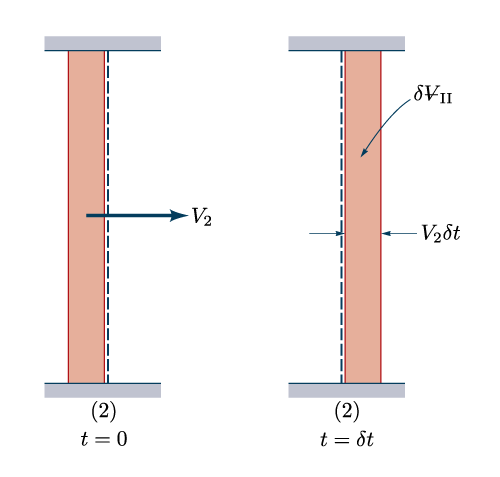
\includegraphics[width=0.4\linewidth]{outflow of B.png}
\end{center}
\end{itemize}
\textbf{Putting it all together}\\
Substituting the previous results into the forward finite difference approximation of the time rate of change of $B$ for the system:
\[\frac{\delta B_{\mathrm{sys}}}{\delta t} = \frac{B_{\mathrm{c\vol}}(t+\delta t)-B_{C\vol}(t)}{\delta t} - \frac{B_{\mathrm{I}}(t+\delta t)}{\delta t} + \frac{B_{\mathrm{II}}(t+\delta t)}{\delta t}\]
We get:
\[\boxed{\frac{DB_\text{sys}}{Dt} = \frac{\partial B_{C\vol}}{\partial t} - \dot{B}_{\text{in}} + \dot{B}_{\text{out}}}\]
Or equivalently:
\[\boxed{\frac{DB_\text{sys}}{Dt} = \frac{\partial B_{C\vol}}{\partial t} - (\rho_1 b_1 A_1 V_1) + (\rho_2 b_2 A_2 V_2)}\]
\hl{This is the \textbf{restrictive form of Reynolds transport theorem} valid for a fixed control volume with one inlet and one outlet, uniform flow properties across each section, and velocity normal to the inlet and outlet surfaces.} We will generalize this equation in the following section.
\subsection*{Generalized Reynold's Transport Theorem}
So far, we have derived the Reynolds Transport Theorem for uniform flow perpendicular to the inlet and outlet surfaces. However, in general, the flow properties may vary across the control surface and the flow may not be perpendicular to it.\\\\
Thus, we can start by considering a small area element $\delta A$ on the control surface. The fluid velocity normal to this surface is 
\[V_n = V\cos\theta = \vec{V} \cdot \hat{n}\]
Where $\hat{n}$ is the outward unit normal vector to the control surface and $\theta$ is the angle between the velocity vector and the outward normal.
\begin{center}
    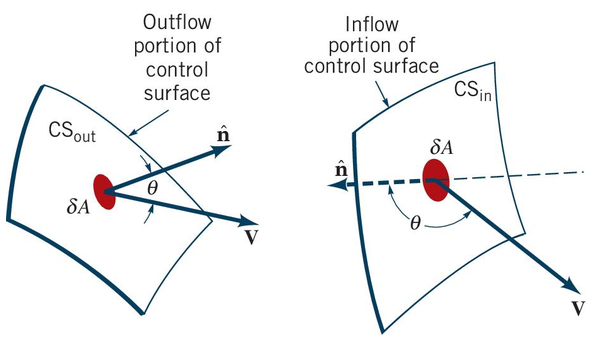
\includegraphics[width=0.5\linewidth]{inflow outflow.png}
\end{center}
The volume that crosses this area element during a small time interval $\delta t$ is:
\[\delta \vol = V_n \delta t \delta A\]
Following the same logic as previously, the rate at which the extensive property $B$ crosses this area element is:
\[\delta B = \rho b \delta \vol = \rho b V_n \delta t \delta A\]
\[\implies \delta \dot{B} = \rho b V_n \delta A\]
Thus, integrating over the outflow portion of the control surface, 
we can express the total rate of outflow of $B$ as:
\[\dot{B}_{\text{out}} = \int_{CS_{\text{out}}} \rho b (\vec{V}\cdot \hat{n}) \, dA\]
Similarly, the total rate of inflow of $B$ is:
\[\dot{B}_{\text{in}} = \int_{CS_{\text{in}}} \rho b (\vec{V}\cdot \hat{n}) \,dA\]
We can combine these two integrals into a single flux integral over the entire control surface:
\[\dot{B}_{\mathrm{out}}-\dot{B}_{\mathrm{in}}=\int_{CS}\rho b(\vec{V}\cdot\hat{n})\,dA\]
This is analogous to Gauss's law in electromagnetism, where a single surface integral over a closed surface represents the net flux of a vector field. Here, the dot product with $\hat{n}$ automatically accounts for the \hl{positive contributions from outflow and negative contributions from inflow (sign convention)}.\\\\
Combining these results, and substituting $B_{C\vol}= \int_{C\vol} \rho b \, d\vol$ we can express the generalized Reynolds Transport Theorem as:
\[\frac{DB_{\text{sys}}}{Dt} = \frac{\partial}{\partial t} \int_{C\vol} \rho b \, d\vol + \int_{CS} \rho b (\vec{V}\cdot \hat{n}) \, dA\]
Now, this equation is valid for any fixed control volume, with arbitrary flow directions and nonuniform flow across the control surface. \hl{But we can push the generalization even further by allowing the control volume to move and deform with time!}\\\\
We simply do this by considering the \hl{relative velocity of the fluid with respect to the control surface}, which results in our grand finale:
\[\boxed{\frac{DB_{\text{sys}}}{Dt} = \frac{\partial}{\partial t} \int_{C\vol} \rho b \, d\vol + \int_{CS} \rho b (\vec{V}_{\text{rel}}\cdot \hat{n}) \, dA}\]
Where $\vec{V}_{\text{rel}} = \vec{V} - \vec{V}_{CS}$ is the relative velocity of the fluid velocity with respect to the control surface velocity. For example:
\begin{center}
    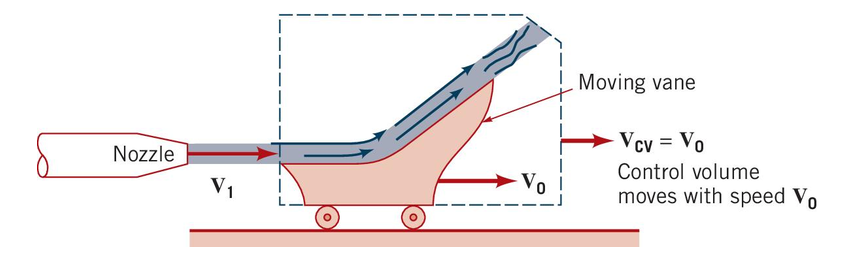
\includegraphics[width=0.8\linewidth]{moving cv.png}
\end{center}
\hl{In summary, the Reynolds Transport Theorem relates the rate of change of an extensive property $B$ (which depends on the mass of the system) as we follow a fluid system along its pathlines to its accumulation within a chosen control volume and its \textit{net transport} across the control surface.} The volume integral represents the accumulation of $B$ within the control volume, while the surface integral represents its net outward flux, with outflow positive and inflow negative by sign convention.\\\\
\textbf{Note on the Rate of Change of the Volume Integral}\\
The first term on the right-hand side of the Reynolds Transport Theorem represents the time rate of change of the extensive property $B$ within the control volume. There are a few notable ways for this term to be nonzero:
\begin{itemize}
\item The control volume is fixed, but the fluid properties $\rho$ and/or $b$ change with time. Since the integration region is constant, we can bring the partial derivative inside:
\[\frac{\partial}{\partial t} \int_{C\vol} \rho b \, d\vol = \int_{C\vol} \frac{\partial(\rho b)}{\partial t} \, d\vol = \int_{C\vol} b\frac{\partial\rho}{\partial t} \, d\vol + \int_{C\vol} \rho\frac{\partial b}{\partial t} \, d\vol\]
The amount of property per unit volume changes with time, even though the control volume remains fixed.
\item The control volume deforms, changing its total volume with time, while the fluid properties $\rho$ and $b$ remain constant. Since the integration region itself changes with time, we use the total derivative:
\[\frac{d}{dt} \int_{C\vol(t)} \rho b \, d\vol = \rho b \frac{d}{dt} \int_{C\vol(t)} d\vol = \rho b \frac{d\vol_{C\vol}}{dt}\]
\end{itemize}
Note that both of these cases can occur simultaneously, in which case we would generally need to evaluate a time-dependent triple integral to account for all the changing variables. However, in most applications, we can make reasonable assumptions about the control volume or fluid properties to simplify the analysis. Typically, we can choose a fixed control volume such that the accumulation term vanishes under steady-flow conditions.\\\\
Also note that there are special cases where the surface integral equals zero (equal rates of inflow and outflow), but the volume integral is nonzero (unsteady flow).\\\\
\textbf{Choosing a Control Volume}\\
Choosing a control volume is analogous to choosing a free-body diagram to analyze in mechanics. Any control valid is theoretically valid, but a good choice can simplify the analysis.\\\\
Generally we want to choose a control volume such that
\begin{itemize}
    \item \textbf{Place unknowns on the control surface,} rather than inside the control volume so that they appear explicitly in the surface integral terms.
    \item \textbf{Choose control surfaces perpendicular to the flow at inlets and outlets,} so that the dot product $\vec{V}\cdot\hat{n}$ simplifies to $\pm V$.
    \item Use simple geometries and surfaces to simplify the evaluation of the integrals.
\end{itemize}
The intuition is to choose a control volume so that the unknown quantities appear naturally in the equations while minimizing the complexity of everything else.
\begin{center}
    {\LARGE\bfseries Finite Control Volume Analysis\par}
\end{center}
In this chapter, we will explore the ways to apply the Reynolds Transport Theorem to analyze fluid flow through a control volume. The big idea is to use laws of conservation where the material derivative of an extensive property $B$ has a known equality, such as $DM/Dt=0$ for mass conservation, $D\vec{P}/Dt=\sum \vec{F}$ for momentum conservation and then solve the right-hand side of the Reynolds Transport Theorem to determine the unknowns.
\section*{\fbox{5.1 Conservation of Mass (Continuity Equation)}}
\addcontentsline{toc}{section}{5.1 Conservation of Mass (Continuity Equation)}










\end{document}
